\documentclass[11pt]{article}
\usepackage{fec}
\usepackage{mathtools}
\usepackage{longtable}
\usepackage{array}
\usepackage{graphicx}
\usepackage{lscape}
\usepackage{verbatim}
\usepackage{amsmath}

\begin{document}
\title{Complexity of Pivot Algorithms}
\author{Qi Wang, Sean Kelley}
\date{December, 2020}
\maketitle


\begin{abstract}
Abstract...
\end{abstract}


\section{Introduction}
Simplex method was invented by Dantzig in 1947 \cite{dantzig1951maximization} to solve the Linear Optimization (LP) problem. It was tableau pivoting based method and pivoting under certain rules. The rules can be flexible so many simplex variants have been developed afterwards. Another framework of pivot algorithm is criss-cross method, which was proposed by Zionts at 1969 \cite{fukuda1997criss} and then \cite{terlaky1987finite}, \cite{chang1979least} present finite criss-cross version independently around 1980s. Some variant pivot methods appeared by proposing different pivots rules. We will describe them in the following section. \textbf{Mention Short simplex paths}\\
Although simplex method was generally efficient in practical, theoretically, Klee and Minty \cite{wikipediacontributors_2020_kleeminty} in 1970s showed the worst case that, a specific type of LO problem, a variant of simplex method visited all vertices (exponential steps) until solve the problem to be optimal. The feasible region of such problems was call Klee-Minty cube whose corners have been "squashed". We will demonstrate some examples in the following section. For now, it is still an unaccomplished problem that to design a pivot algorithm and prove that the number of pivot steps is bounded by polynomial of number of variables and constraints.
The paper is structured as follows: in Section 2 we define the LO problem, list the notation and (\textbf{might present some algorithms}); in section 3 we discuss the complexity of pivot algorithms and give a brief conclusion in the final section.

\section{The pivot algorithm for LO}
In this paper, we consider the Linear optimization problem of the standard form
\begin{align}
\begin{split}
\min \quad &c^Tx\\
\text{s.t.} \quad &Ax = b\\
&x \ge 0\\
 x \in \Rmbb^n,\ c \in \Rmbb^n,\ &A \in \Rmbb^{m\times n},\ b \in \Rmbb^m   
\end{split}
\end{align}
\begin{table}[h]
\caption{Notation}
\centering
\begin{tabular}{lll}
\hline
$n$ & number of variables   &  \\
$m$ & number of constraints (assume $m \le n$) &  \\
\hline
\end{tabular}
\end{table}
\section{Complexity - worst case}
Given $m$ constraints and $n$ variables, there are at most $\binom{n}{m}$ possible basis, which is a upper bound for the number of iterations for pivot algorithms. When $m=\frac{n}{2}$, $\binom{n}{m}$ get its maximum $\binom{n}{\frac{n}{2}}\approx \sqrt{\frac{2}{\pi n}}2^n$. Klee and Minty defined a type of LO problems which many pivot algorithms will visit all the vertices to find the optimal solution. Detailed introduction of Klee Minty cube can be referred to \cite{vanderbei2020linear}. Here we demonstrate some simple examples. For such problem
\begin{align*}
\max &\sum_{j=1}^n 2^{n-j}x_j\\
\text{s.t. } &2\sum_{j=1}^{i-1}2^{i-j}x_j + x_i \le 5^i &i=1,\cdots,n\\ 
			&x_j \ge 0 & j=1,\cdots,n
\end{align*} 
When $n=2$ and $n=3$ the 2-d and 3-d Klee Minty LO problems are 
\begin{align*}
\begin{split}
\max \quad & 2x_1 + x_2 \\
\text{s.t. }\quad  & x_1 \le 5\\
& 4x_1 + x_2 \le 25\\
& x_1 \ge 0,\ x_2 \ge 0.
\end{split}
\begin{split}
\max \quad & 4x_1 + 2x_2 + x_3 \\
\text{s.t. }\quad  & x_1 \le 5\\
& 4x_1 + x_2 \le 25\\
& 8x_1 + 4x_2 + x_3 \le 125\\
& x_1 \ge 0,\ x_2 \ge 0, \ x_3 \ge 0.
\end{split}
\end{align*}
The feasible region of 2-d Klee Minty problem is showed in Figure \ref{fig:test}. And the feasible region of 3-d problem is shown in \textbf{TO be added}. 
\begin{figure}
{\caption{Feasible region of 2-d Klee Minty cube with contour lines.}\label{fig:test}}
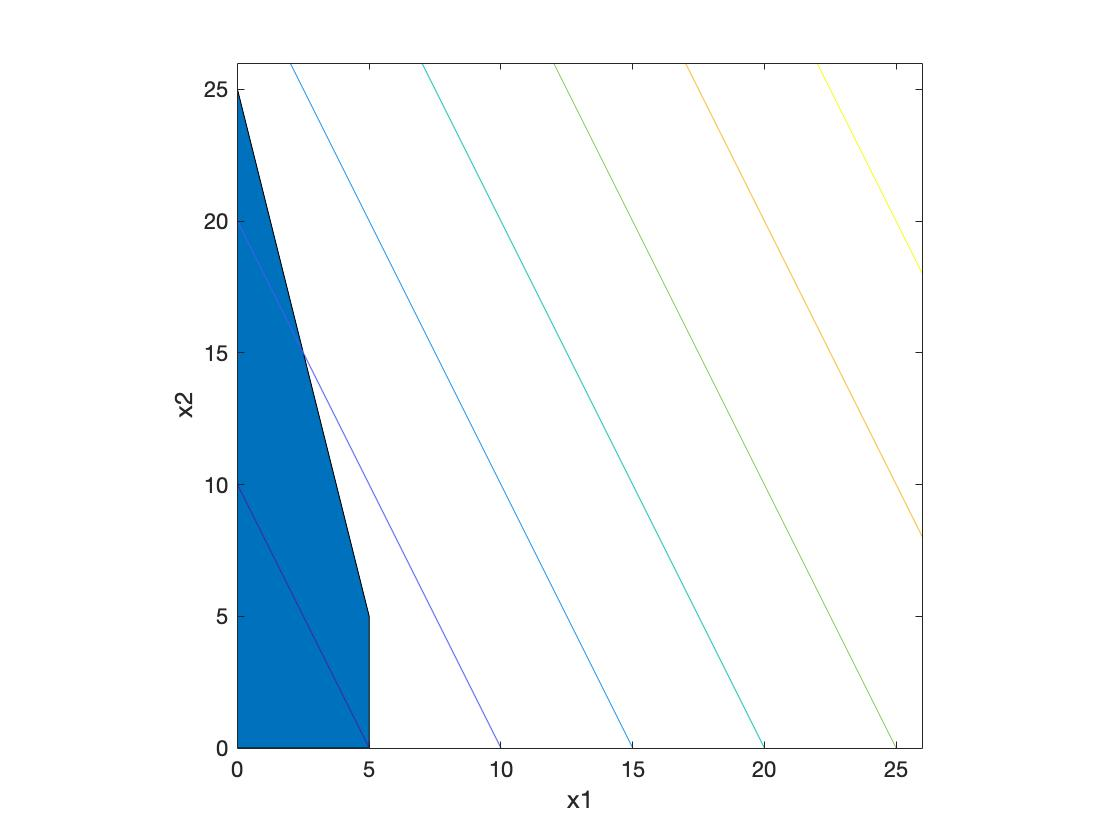
\includegraphics[scale=0.30]{klee_cube_d2.jpg}
\end{figure}
Let's apply primal simplex method with least-index and Dantzig (choose the biggest reduced cost) pivot rules to demonstrate the number of pivot steps.
\textbf{To be nicer table}
\begin{figure}[h]
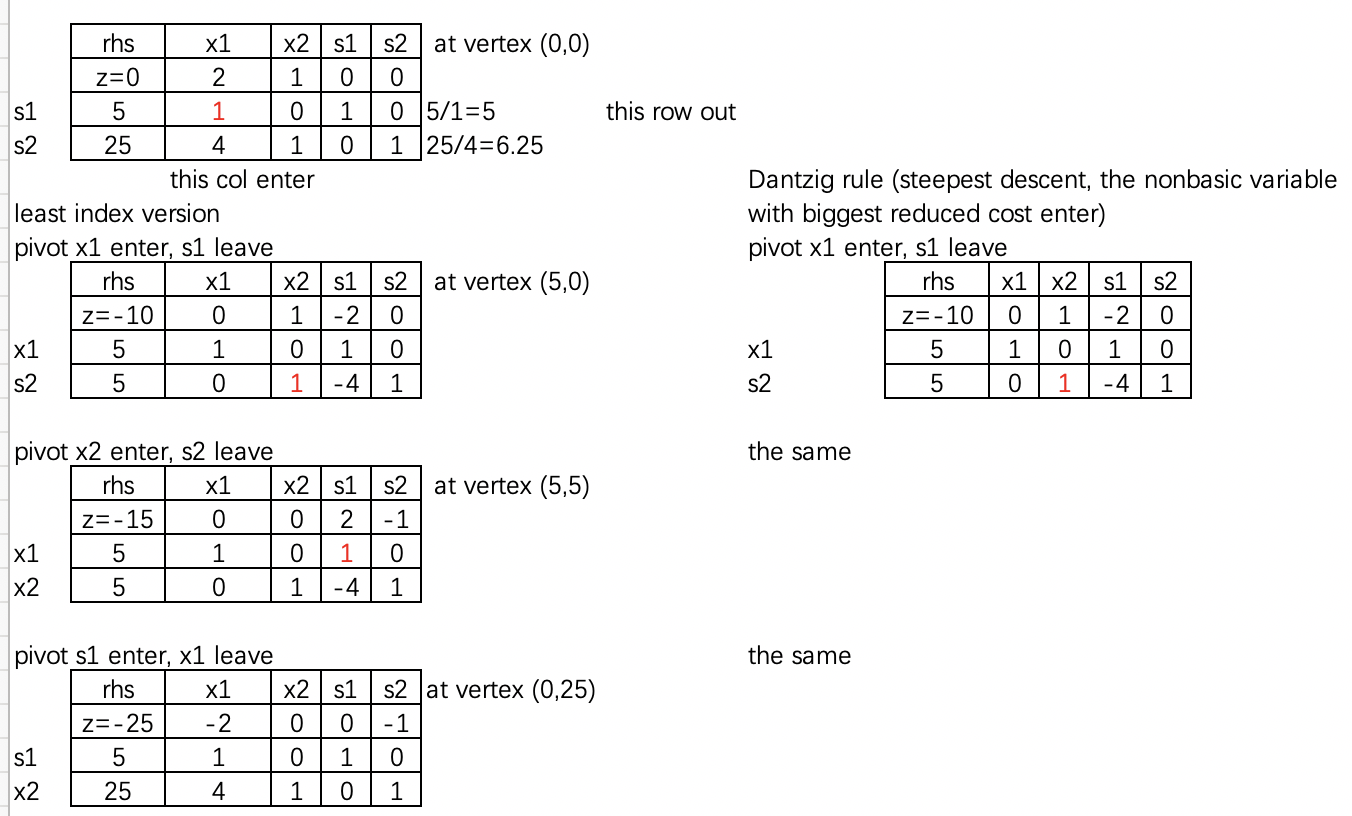
\includegraphics[scale=0.50]{klee_pivot.png}
\end{figure}
%\section{title}
%There are certain pivot rules:
%\begin{itemize}
%\item Bland's rule, lexicographic rule
%\item Clairvoyant pivot rule (only theoretical), unimplementable
%\item Hirsch conjecture : disproven by Francisco Santos, 2011
%\item Polynomial Hirsch conjecture -- still open
%\end{itemize}


\section{Conclusion}
Conclusion...

\bibliographystyle{plain}
\bibliography{reference.bib} 

\end{document}
